\textbf{Definition:} Das Schweissen ist das schmelzflüssige Vereinigen 
von Werkstoffen in der Schweisszone unter Anwendung von Wärme 
und/oder Kraft mit oder ohne Schweisszusatz.\\

\begin{minipage}{0.5\linewidth}
    \begin{center}
        \textbf{WIG}
    \end{center}
    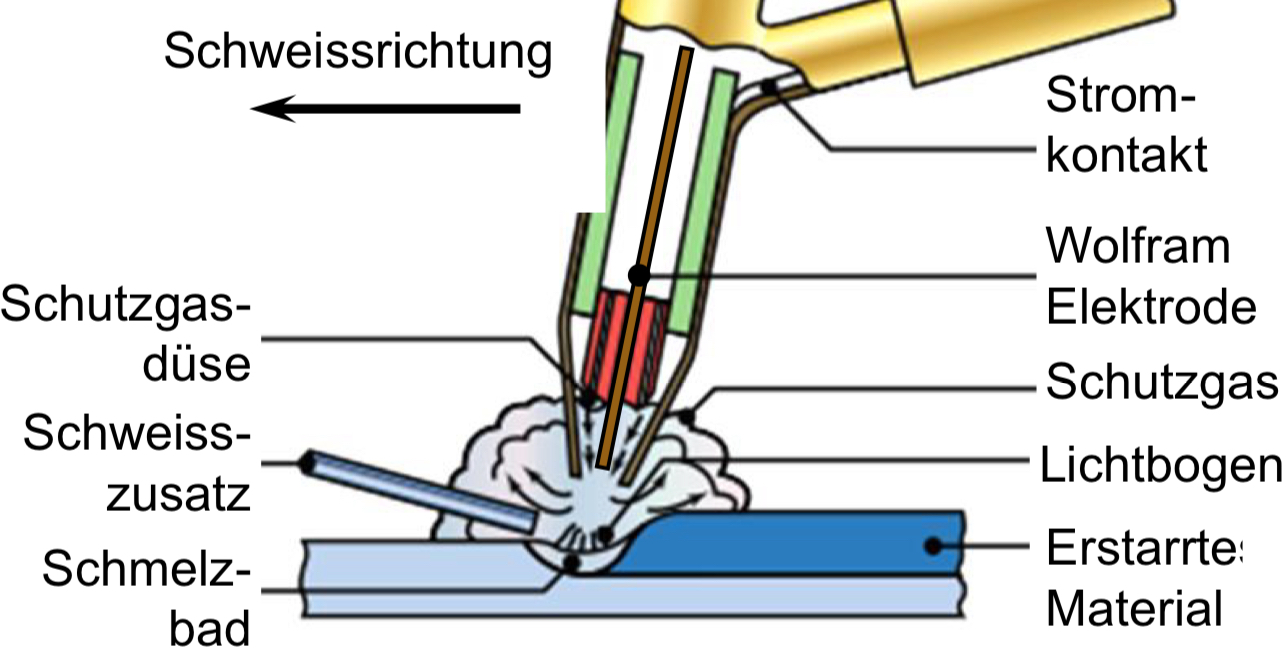
\includegraphics[width=\linewidth]{src/images/WIG.jpeg}\\
\end{minipage}
\begin{minipage}{0.5\linewidth}
    \begin{center}
        \textbf{MSG}
    \end{center}
    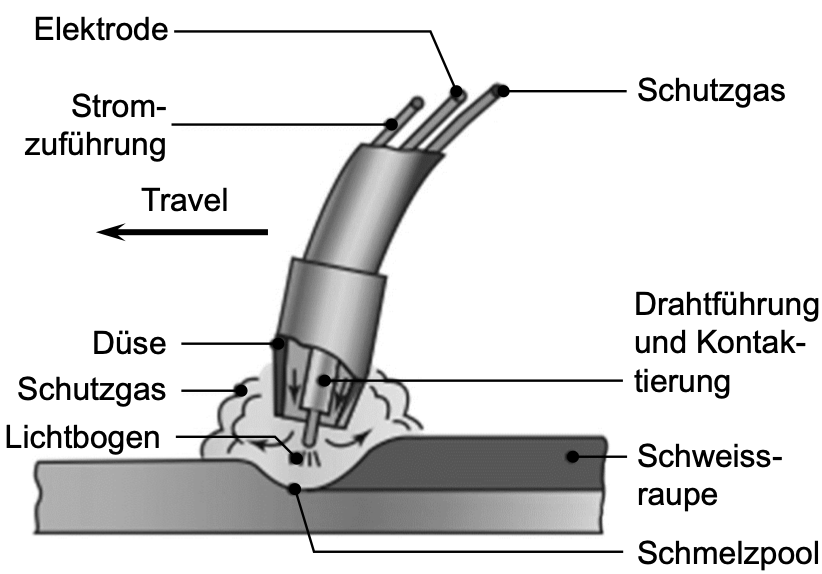
\includegraphics[width=\linewidth]{src/images/MSG.png}\\
\end{minipage}
\textbf{WIG:} Verwendet einen Gleichstromlichtbogen. 
Wolframelektrode hat negative Polarität und fungiert als Kathode. 
Das Werkstück ist die Anode. \\

\textbf{MSG (MIG/MAG) Schweissen:} Bei niedriger Spannung und Strommstärke 
treten Spritzer auf. Es wird kontrolliert zwischen globularem Materialübergang 
und Sprühtransfer gewechselt, um einzelne Tropfen zu übertragen. \\

\textbf{Plasmaschweissen:}\\
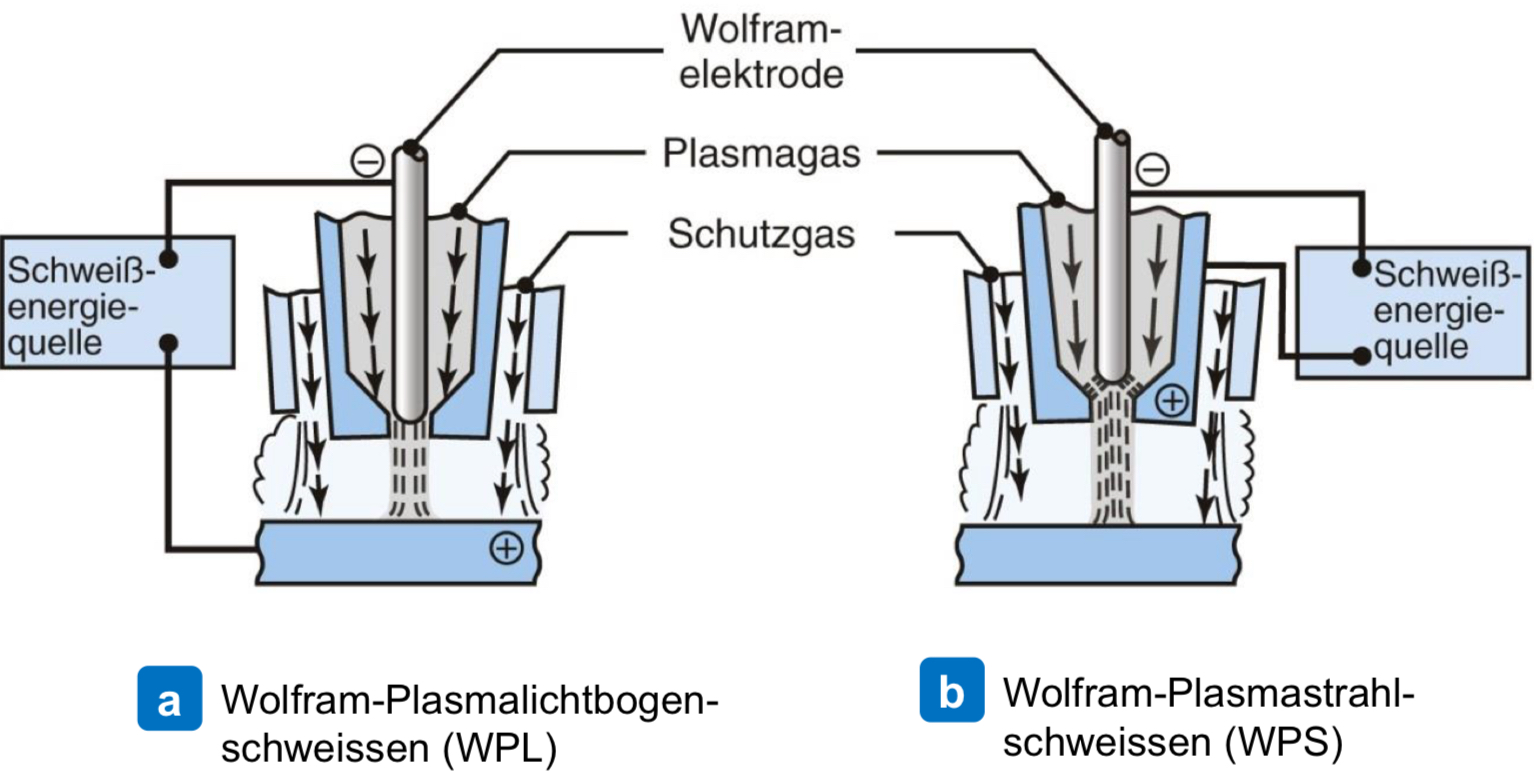
\includegraphics[width=0.8\linewidth]{src/images/WP.jpeg}\\

\textbf{Cold Metal Transfer (CMT):} Draht wird mit 50-130 Hz hin und 
her bewegt. CMT erkennt einen Kurzschluss und zieht Draht zurück. 
Vorteile sind kontrollierte und spritzerfreie Materialablagerung, 
geringe Wärmeeinwirkung und gute Energieeffizienz.\\

\textbf{Gleich- und Wechselstromschweissen:} Beim Gleichstromschweissen 
und negativ gepolter Elektrode ergeben sich die längsten 
Elektrodenstandzeiten. Im Werkstück bildet sich eine Art Kegel. 
Beim Wechselstromschweissen fliessen die Elektronen vom Werkstück 
zur Elektrode und reissen dabei die hochschmelzende Oxidschicht auf. 
Im Werkstück bildet sich eine Art Erhebung.\\

\textbf{Impulsschweissen:} Strom wird in Impulse unterteilt, weniger Wärme ins Material\\
"gezielt zwischen
globularem Materialübergang und Sprühtransfer
gewechselt, um einzelne Tropfen zu übertragen" - whatever\\
\vfill \null \columnbreak

\textbf{Auslegung Schweissnaht:}\\


\begin{minipage}{0.55\linewidth}
    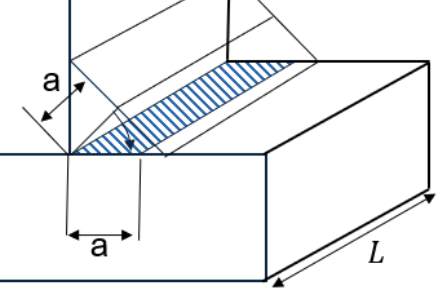
\includegraphics[width=0.8\linewidth]{src/images/Schweissnaht.png}\\
\end{minipage}
\begin{minipage}{0.30\linewidth}
    \[
        \boxed{     
            \begin{aligned}
                \sigma_{eq} &= \frac{F}{A_f}\\
                A_f &= l_{eff} \cdot a\\
                l_{eff} &= L - 2 \cdot a
            \end{aligned}
        }
        \]
\end{minipage}\\

\textbf{Reibschweissen:}\\
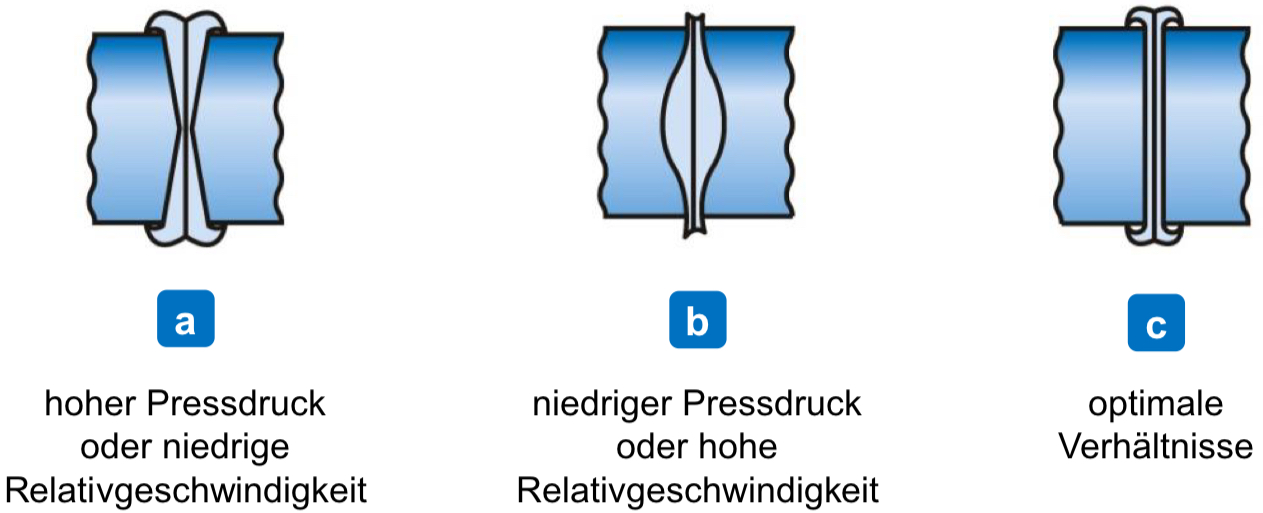
\includegraphics[width=\linewidth]{src/images/Reibschweissen.jpeg} \\

\textbf{Schweissnähte:} \\
Breite und Dicke der Schweissnaht nimmt mit der Drahtvorschubgeschwindigkeit zu.\\

\textbf{Schweissgeschwindigkeit:}\\
\begin{minipage}{0.5\linewidth}
    \[
    \boxed{     
        v_t = \frac{v_w \cdot A_{w}}{\textcolor{ForestGreen}{A_{b}}}
    }
    \]
\end{minipage}
\begin{minipage}{0.5\linewidth}
    \begin{tiny}
    \item $v_{t}$: Schweissgeschwindigkeit
    \item $v_w$: Drahtvorschubgeschwindigkeit
    \item $A_w$: Drahtquerschnitt
    \item $\textcolor{ForestGreen}{A_b}$: Raupenquerschnitt
    \item $\textcolor{red}{A_e}$: Einbrandzone
    \end{tiny}
\end{minipage}\\
\textbf{Schweissraupen:} Querschnittsform mit Parabel approximierbar.\\
Querschnittsfläche aus Kontinuitätsgleichung:\\

\textbf{Schutzgasschweissen Leistung Auslegung:}\\

\begin{minipage}{0.5\linewidth}
    \[
    \boxed{     
        \begin{aligned}
            P &= V \cdot I \cdot \eta \\
            &= V \cdot K \cdot v_{w} \cdot \eta
        \end{aligned}    
        }
    \]
\end{minipage}
\begin{minipage}{0.5\linewidth}
    \begin{tiny}
    \item $P$: Leistung beim Schweissen
    \item $V$: Spannung
    \item $I$: Strom
    \item $\eta$: Wirkungsgrad
    \item $K$: Proportionalitätsfaktor
    \end{tiny}
\end{minipage}\\
\vspace{1mm}


\textbf{Aufmischung D:} 
    \begin{tiny}
 \[
    \boxed{     
        D=\frac{\text{Zusatzmaterial}}{\text{Zusatzmaterial } + \text{ Grundmaterial}} = \frac{A_b}{\textcolor{ForestGreen}{A_b} + \textcolor{red}{A_e}}
    }
    \]
    \end{tiny}\\
Bsp. "80\% Aufmischung" bedeutet, dass 80\% vom Grundmaterial 
und 20\% vom Füllmaterial stammen.\\

\textbf{Schmelzbad:} 
\begin{itemize}
    \item \textbf{DC, Elektrode negativ:} \\Tiefes Schmelzbad, keine Oberflächenreinigung
    \item \textbf{DC, Elektrode positiv:} \\Seichtes Schmelzbad, Oberflächenreinigung
    \item \textbf{AC:} Intermediate
\end{itemize}

\textbf{Störungsfaktoren - Schmelzbad:} Auftrieb, Oberflächenspannung, Lorentzkraft, Scherspannung des Schutzgasstroms\\

\textbf{Fehler in Schweissnähten:} Längsrisse, Querrisse, Kerbrisse, 
Überlappungen, Einrandkerben, Einschlüsse, Porosität, Ungenügende 
Durchschweissung, Nahtunterschreitung, unvollständige Verbindungen. \\
Entstehen durch zu geringen Schutzgasfluss, instabile Keyholes, 
Kontamination der Oberflächen.\\
\includegraphics[width=0.5\linewidth]{src/images/Schäfflerdiagramm.png}
\includegraphics[width=0.5\linewidth]{src/images/Schweissnähte.jpeg}\\


\textbf{Schäfflerdiagramm:} Das Schäfflerdiagramm kann die resultierende 
Phasenzusammensetzung eines Chrom-Nickel-Stahs abgeschätzt werden. 
Dabei berücksichtigt werden Ni, C, Mn, N, Mo, Si, Nb, Ti.\\





